% Generate lecture notes
%
% To generate the table of contents
% pdflatex * 2 is required.

\documentclass[a4paper]{article}
\usepackage{beamerarticle}%
\mode<article>%
\usetheme{CambridgeUS}
\usefonttheme{serif}
\usepackage{CJKutf8}
\usepackage[colorlinks,linkcolor=blue,anchorcolor=blue,citecolor=blue]{hyperref}%
\hypersetup{unicode}
\usepackage{bookmark}
\usepackage{graphicx}%
% \usepackage{geometry}
% \geometry{left=2.0cm,right=2.0cm,top=2.0cm,bottom=2.0cm}
\renewcommand{\contentsname}{目录}
% ignores the frame header.
\setbeamertemplate{frametitle}{}
\setbeamertemplate{framesubtitle}{}
\setjobnamebeamerversion{example_beamer}

\begin{document}
\begin{CJK}{UTF8}{song}
    \documentclass[tikz]{standalone}
\usepackage{tikz}
\usepackage{graphicx}
\usepackage{pgfplots}
\pgfplotsset{compat=1.17}
\begin{document}
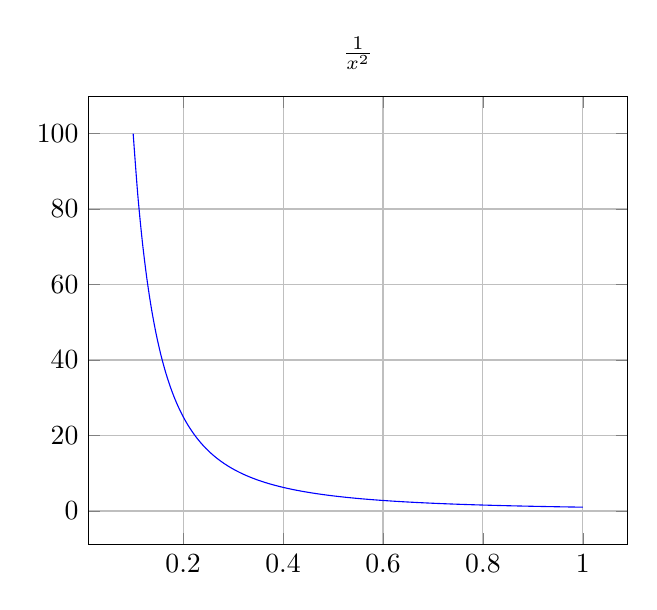
\begin{tikzpicture}
	\begin{axis}[
    title={$\frac{1}{x^2}$},grid=major]
    \addplot [smooth,blue,domain=0.1:1,samples=100] {x^-2};
	\end{axis}
\end{tikzpicture}
\end{document}
\end{CJK}
\end{document}